
\chapter{Prefetching SPARQL Query Cacher}\label{sec:tpfcacheplanning}

\section{Introduction}

This chapter describes an effort to create a proxy that can cache the
results of not only complete SPARQL queries, but also the results of individual
triple patterns. It will asynchronously analyse executed queries, and
may prefetch the results of certain triple patterns into the cache.


\subsection{Scenario}

The system is in the convergence of the directions described in this
thesis: It should relieve the remote endpoint of some of the
burden to evaluate the query and it should add to the robustness of
the open Web SPARQL infrastructure. It uses hypermedia to answer
individual triple patterns, based on Triple Pattern Fragments (TPF)
\cite{ldf1}. The system does not support named graphs (i.e. only
triplestores), but other than that, it supports SPARQL 1.1 in its
entirety. It was possible to develop this quickly by the efforts put
into the query planning in the Attean framework described in
Section~\ref{sec:conpush}. Caching based on RFC7234 \cite{rfc7234} was
shown to be of possible use in the survey I conducted. Finally, it was
planned to be evaluated using Design of Experiments.

Unfortunately, the system has as of this writing insufficient
performance for an evaluation to be meaningful. Nevertheless, it
points out some interesting lessons with varying degrees of
certainty. This chapter will detail the system, show its design and
features and discuss its strengths and weaknesses.

Figure~\ref{fig:messaging} illustrates where caches may be in the
Internet infrastructure, as well as HTTP requests and responses in a
typical deployment scenario of the system.

\begin{figure}
\begin{center}
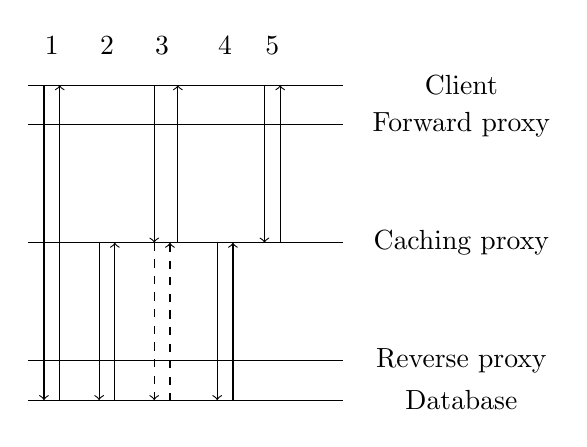
\begin{tikzpicture}
\draw (0,0) --(4,0);
\node at (5.5,0) { Database };
\draw (0,0.5) --(4,0.5);
\node at (5.5,0.5) { Reverse proxy };
\draw (0,2) --(4,2);
\node at (5.5,2) { Caching proxy };
\draw (0,3.5) --(4,3.5);
\node at (5.5,3.5) { Forward proxy };
\draw (0,4) --(4,4);
\node at (5.5,4) { Client };

\draw [->] (0.2,4) --(0.2,0);
\draw [<-] (0.4,4) --(0.4,0);
\node at (0.3,4.5) {\circled{1}};
\draw [->] (0.9,2) --(0.9,0);
\draw [<-] (1.1,2) --(1.1,0);
\node at (1.0,4.5) {\circled{2}};
\draw [->] (1.6,4) --(1.6,2);
\draw [dashed, ->] (1.6,2) --(1.6,0);
\draw [dashed, <-] (1.8,2) --(1.8,0);
\draw [->] (1.9,2) --(1.9,4);
\node at (1.7,4.5) {\circled{3}};
\draw [->] (2.4,2) --(2.4,0);
\draw [<-] (2.6,2) --(2.6,0);
\node at (2.5,4.5) {\circled{4}};
\draw [->] (3,4) --(3,2);
\draw [->] (3.2,2) --(3.2,4);
\node at (3.1,4.5) {\circled{5}};
\end{tikzpicture}
\caption{The possible positions of a cache. A cache may reside at both
  the server side (as a database cache) or client side, or any of the
  intermediate proxies. The arrows illustrate requests (when pointing
  down) and responses (when pointing up) in a deployment scenario for
  when the query cache considered in this paper is deployed on a
  caching proxy in the Internet infrastructure (see the text for
  details).}\label{fig:messaging}
\end{center}
\end{figure}

The system is based on HTTP, which implies a client-server
architecture. In this architecture, a cache may be present at
conceptually five different levels. First, the client may have its own
cache, which caches only responses made by the client itself. The next
level is known as a forward proxy. They aren't currently very common,
but have in the past often been institutional proxies, or proxies
employed by Internet Service Providers for caching responses that may
be common to many of their users. The next level, generically referred
to as a caching proxy, may be in the Internet
infrastructure. Currently, the most common form of this type of proxy
is known as a Content Delivery Network (CDN). It is very common to
have a reverse proxy near the server. They are often known as a ``Web
Accelerator''. Usually, they will communicate with the server with
HTTP, but it is conceivable that it may use a different protocol, and
may employ detailed knowledge of the hosted data to optimise cache
operations. Finally, the database, in this context a SPARQL Endpoint,
may use conventional database caching techniques. The database cache
and reverse proxy are typically controlled by the data provider.

The present system may be deployed at any of these levels (and similar
figures could be drawn). However,
since the database and the reverse proxy in front of it may have
detailed knowledge of the data, e.g. a complete data profile with
statistics to optimise join order, these levels have much in common
with a conventional database cache, which is extensively discussed in
the literature.

My interest is the case where the caching proxy has no further
knowledge of the data than what is exposed through the SPARQL Endpoint
or hypermedia metadata. While this would be known as a mediator in the
database literature and has also been a field of study for 20 years, I
focus on a practical motivation stemming mainly from what is currently
available. In current practice, very little information is available
to the mediator. Also, this study is also practically restricted to
HTTP. If the cache is to be shared, then it would typically reside on
the forward proxy, or in a CDN.

It is further interesting to note the contrast to the HERMES
\cite{adali1996query} system's concept of invariants discussed in
Section~\ref{sec:relcache}: a SPARQL query cache be oblivious
to domain knowledge in a CDN deployment and therefore shouldn't assume any invariants,
except in the possible but unlikely case where the remote server
declares an infinite freshness lifetime for the result of a certain
graph pattern. A forward proxy, on the other hand, may have a deeper
understanding on the needs of the client, and could possibly implement
invariants. The Attean framework accommodates for this.

Figure~\ref{fig:messaging} illustrates the case where HTTP messages
are being passed, where the cache is assumed to reside on a
intermediate caching proxy in the Internet, i.e. a CDN. The figure
may be viewed as having time on the $x$-axis, with the arrows pointing
down being requests and the arrows point up being responses. In this
example, the client first makes a request (request \circled{1}), which
is passed through the proxy because it has not yet cached any
responses. The response (response \circled{1}) is then also
transmitted directly from the SPARQL Endpoint at the database back to
the client. The entire response may be cached on the proxy in case it
can be reused in its entirety. However, the main point is that the
request will be analysed by the proxy in parallel to being sent to the
server, and another request \circled{2} for a triple pattern fragment
that the analyser thinks will enable the proxy to assist the server
the best for future requests, is sent. This analysis is discussed in
Section~\ref{sec:analpre}. The response \circled{2} is not sent back
to the client, but will enter the cache. Assuming that the analyser
was successful and that the cache can be used to answer request
\circled{3}. In that case, the proxy will send rewritten queries for
the rest of the data it needs to be able to answer the query to the
origin server, indicated by the dashed arrows. This may be zero or more SPARQL
query, TPF requests or a combination thereof, depending on what the
planner finds least expensive. The proxy will then evaluate the entire
query and send the final result back as response \circled{3}. In
addition, the analyser may have identified another Triple Pattern
Fragment that it takes as likely to be useful for future requests, and
sends a request and caches the response \circled{4}. At some point, it
may be able to answer the entire query using only cached results, as
illustrated by request and response \circled{5}.

Finally note that in this text, the term Triple Pattern Fragment (TPF)
is understood as a specialisation of Linked Data Fragments (LDF), in
which a Triple Pattern Fragment server must be able to answer any
triple pattern, whereas for a Linked Data Fragments server, this is
not required. However, there is no difference in the current
implementation, so in practice, the terms could be used
interchangeably.


\subsection{Architecture}\label{sec:arch}

The architecture is depicted in Figure~\ref{fig:arch}. A SPARQL
protocol implementation will accept a client's query (and could cache
it's result in its entirety, but this is neither implemented nor
depicted). Two things happen to a valid query:

\begin{itemize}
\item The query (or indeed the algebra) is sent asynchronously to a
  set of analysers that is tasked with predicting what parts of the
  incoming query may be useful to answer future queries. The result of
  the analysis is sent to a prefetcher that will decide how to fetch
  the needed data, currently it only operates on triple patterns, and
  therefore, and since it is also assumed that a triple pattern
  fragments server can answer any triple pattern, it instructs a TPF
  client to fetch and enter the result into the cache.  
\item The SPARQL protocol implementation will also send the query to
  a parser that will create an algebra tree from it. The algebra tree
  is then passed to a query engine for immediate execution. The query
  engine has an elaborate query planner that can create plans for
  accessing a cache, a TPF server and a SPARQL Endpoint. When the
  planner finishes planning, the evaluator may use a TPF client or a
  SPARQL protocol client to fetch data that is not in the cache. The
  results of single triple patterns may be inserted in the cache by
  the TPF client.
\end{itemize}

\begin{figure}[h!]
\begin{center}
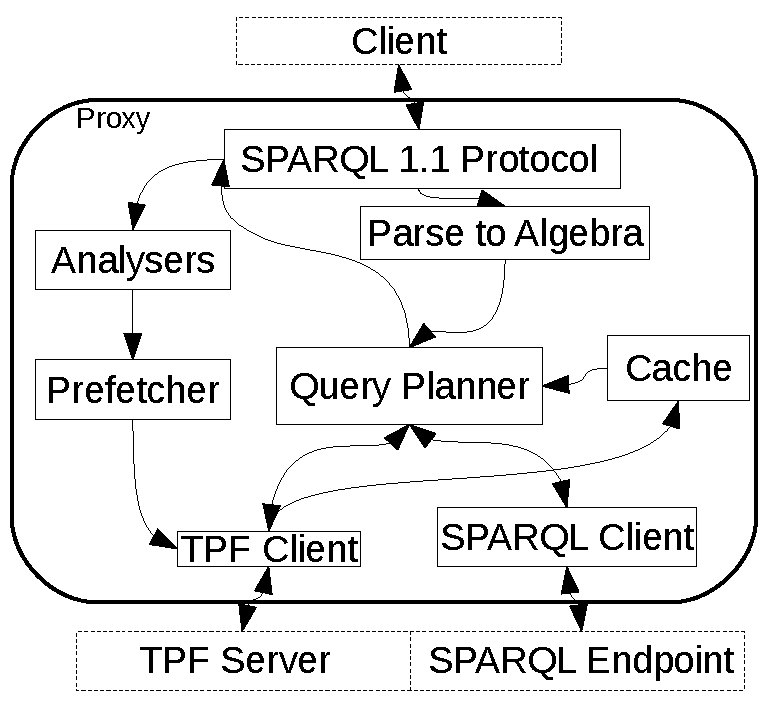
\includegraphics{architecture.pdf}
\caption{Architectural overview. The proposed system is represented
  inside the box titled ``Proxy''. It interacts with a client, a
  Triple Patterns Fragments Server and a SPARQL Endpoint. The most
  important components are the query engine, which consists of a query
  planner and a query evaluator, and the analysers that find
  subqueries to cache.}\label{fig:arch}
\end{center}
\end{figure}


\subsection{Understanding the Query Planning}\label{sec:understandquery}

We saw in Section~\ref{sec:introinteract} that a query would be parsed
to a tree of algebra objects and then a query planner would traverse
the algebra tree to create a plan tree by finding all the ways the
data can be accessed, or operations executed over them. For example,
if the input query has a BGP with two triple patterns and there are
two types of join operations, it may result in four trees, where each
of the join operation plans are paired with both access plans for the
triple patterns.

It is next the query planner's task to determine which of the possible
plans it should execute. A common choice to perform this task is to
estimate the cost executing various choices.

The resulting plan trees may be represented as strings as follows:
\begin{example}{Four Attean plan trees}
\begin{verbatim}
- Hash Join { s } (distinct cost: 27)
-   Quad { ?s, <http://example.org/p>, ?o, <http://example.org/> } (cost: 15)
-   Quad { ?s, <http://example.org/p>, "1", <http://example.org/> } (cost: 12)

- Hash Join { s } (distinct cost: 28)
-   Quad { ?s, <http://example.org/p>, "1", <http://example.org/> } (cost: 12)
-   Quad { ?s, <http://example.org/p>, ?o, <http://example.org/> } (cost: 15)

- NestedLoop Join (distinct cost: 180)
-   Quad { ?s, <http://example.org/p>, "1", <http://example.org/> } (cost: 12)
-   Quad { ?s, <http://example.org/p>, ?o, <http://example.org/> } (cost: 15)

- NestedLoop Join (distinct cost: 180)
-   Quad { ?s, <http://example.org/p>, ?o, <http://example.org/> } (cost: 15)
-   Quad { ?s, <http://example.org/p>, "1", <http://example.org/> } (cost: 12)
\end{verbatim}
\end{example}
In the above example, the first plan tree will be returned from the
query planner for execution, since it has the lowest estimated cost
(27). Since the SPARQL engine operates over quads, we have assigned a
dummy graph name when constructing the Model, namely
\rdfterm{<http://example.org/>}. 


The system we propose is based on this paradigm, any choices we make
are therefore to be encoded into a cost model. The cost model itself
is not considered a part of the contributions, it is a simple cost
model based on heuristics that arises from the following
discussion. The heuristics themselves are best considered an
implementation detail and is described in
Section~\ref{sec:costheuristics}.

Recall Problem~\ref{prob:cachecartesian}, where a BGP with three
triple patterns could break into two components if the triple pattern
connecting the two others was cached. It is one of the requirements
for the heuristics of the cost model that it is be able to avoid such
situations.

As mentioned, the proposed query planner takes may access a remote
SPARQL endpoint and a Linked Data Fragments Server as well as the
local cache. I have also said that a key motivation behind the study
is to relieve the remote endpoint of load. It was argued in
\cite{verborgh2014querying} that LDF shifts the burden of query
evaluation to the client, and so relieves the server of load. It is
not clear from the literature that this strikes the right balance, it
is my belief that the balance must depend on the concrete server and
client capabilities, keeping in mind
Problem~\ref{prob:microcontroller}. Future work to determine the right
balance in a given situation would be welcome in this area, but I
believe it would be advantageous to build on a cost model.

Following this discussion, consider this example:
\begin{example}{A four-triple pattern BGP}\label{ex:bgp4}
\begin{verbatim}
?s <http://example.org/m/p> "1" ;
   <http://example.org/m/q> <http://example.org/m/a> ;
   <http://example.org/m/p> ?o .
?o <http://example.org/m/b> "2" .
\end{verbatim}
\end{example}
Say that the first triple pattern has a result in the cache. This will
not cause Problem~\ref{prob:cachecartesian} to occur (it would have
occurred if the third triple pattern had a cached result, however), so
we can safely use the cache. The results of the three remaining triple
patterns must be fetched from a remote server. There are essentially
two reasonable choices: Either fetch the result from an LDF server as
argued by \cite{verborgh2014querying} and join them locally or send a
single, rewritten SPARQL query to the remote endpoint for the
evaluation. When the results are returned from both the cache and the
remote endpoint, they must then finally be joined to produce the final
result returned to the client. A string representation of the plan
tree from the current implementation reflects this and reads (note
that accessing the cache is represented by an iterator plan):
\begin{example}{An example Attean plan with a remotely executed BGP}
\begin{verbatim}
- Hash Join { s } (distinct cost: 74)
-   SPARQLBGP (cost: 60)
-     Quad { ?s, <http://example.org/m/p>, ?o, <http://test.invalid/graph> }
-     Quad { ?o, <http://example.org/m/b>, "2", <http://test.invalid/graph> }
-     Quad { ?s, <http://example.org/m/q>, <http://example.org/m/a>, <http://test.invalid/graph> }
-   Iterator (?s with 2 elements) (cost: 2)
\end{verbatim}
\end{example}

Merging the quad plans into a single SPARQL BGP plan is not
straightforward in the presence of a quad pattern that is to be looked
up in e.g. a cache. If we assign the letters $A$, $B$, $C$ and $D$ to
quad patterns \todo{correctly expressed?} in the order in
Example~\ref{ex:bgp4}, the initial join tree produced by parsing may
be $ ((A \bowtie B )\bowtie C) \bowtie D) $. Now, we are interested in
a plan on the form $A \bowtie BCD$, i.e. $BCD$ is reduced to a more
fundamental plan type, in this example a SPARQL BGP. This will
minimise the number of HTTP requests, in much the same way as the
exclusive groups of
\cite{springerlink:10.1007/978-3-642-25073-6-38}. To facilitate this,
we employ \emph{join rotation}. A simple example of join rotation
would be this: We first generate subplans for both $((A \bowtie B
)\bowtie C) \bowtie D) $ and $ (A \bowtie B )\bowtie (C \bowtie D)
$. Then, $C$ and $D$ can be merged to a SPARQL BGP to $ (A \bowtie B
)\bowtie CD $. Another rotation can then be performed: $ A \bowtie (B
\bowtie CD) $ and then coalesced to the final result. The planner will
generate alternative plans for both rotated and unrotated plans, and
all generated plans are subject to cost estimation, so whether a large
BGP plan will be evaluated remotely, or as a join of local cached
results and a smaller remote BGP, or a remote Triple Pattern Fragments
server, is up to the cost estimation. This will be discussed in detail
in Section~\ref{sec:costheuristics}.

As can be imagined from the fact that a BGP with just to triple
patterns result in 4 plan trees, a naive query planner may generate a
large number of plans for complex queries. In addition, the proposed
system will generate even more plans, since it considers three sources
of the same data, the cache, the remote endpoint and an LDF
server. Various methods have been developed in the literature to limit
the growth of plans. In addition to a naive planner, we also have an
Iterative Dynamic Programming planner
\cite{Kossmann:2000:IDP:352958.352982}, which prunes plans
aggressively based on their estimated cost in each iteration of query
plan generation.

\subsection{Analysis for prefetching}\label{sec:analpre}

The objective of the analyser in Figure~\ref{fig:arch} is to predict
what remote data is most useful to answer future queries. I haven't
attempted to formalise the notion of what a useful cache entry is, nor
have I attempted to exploit the concept of profitable query patterns
of \cite{papailiou2015graph}, mostly because this work came at a time
where my work was already near the deadline. I opted for a simple
approach to consider only individual triple patterns.

With this constraint, the analysers have been implemented with two
different assumptions of usefulness: The first analyser, called
predicate-count, captures frequently occurring bound predicates. This is due to the
observation that predicates are often bound, and so predicates that
are common will occur in the future, and therefore, prefetching and
caching results of a triple pattern where the predicate is bound to a
frequently occurring is likely to be beneficial. This is done by
counting the occurrences of predicates, and when the number exceeds a
certain threshold, the prefetcher is instructed to fetch the data.

The second analyser, named cost-reduction, works along a different
axis: It will find the 
triple pattern that, if cached, would provide the greatest cost
benefit. To do so, it will rerun the query planner on the incoming
query while simulating that the results of a certain triple pattern
was in the cache. The simulation will run for \emph{all} triple
patterns that do not already have a cached result. If the cost
reduction of the best plan is larger than a certain limit, the
prefetcher is invoked.



\section{Implementation}\label{sec:impl}

This section explores the implementation of the general architecture
outlined in Section~\ref{sec:arch}. 

The implementation consists of several modules that have been
published to the Comprehensive Perl Archive Network as Free Software,
and most of which have become a part the Free Software ecosystem. For
a detailed account of the modules that are a part of the system and
the authors that have contributed code in this ecosystem, see
Appendix~\ref{sec:modules}. Some parts are essential for the
discussion and to understand the contributions, and therefore detailed
in the following:

\subsection{The Attean Framework}\label{sec:attean}

The Attean framework was born from the experiences the PerlRDF
community gained with \pmodule{RDF::Trine}, the Perl counterpart to
the better known Jena framework, and the opportunities presented by
the introduction of traits \cite{traits}, or roles as they are known
to the Perl world.

Traits are groups of methods that serve as a primitive unit of code
reuse. Traits are not constructed into objects themselves and do not
use inheritance for composition, instead a class is composed by a set
of traits and possibly the class' own methods, and then
instantiated. A trait can also require a set of methods or attributes,
and as such, is similar to an interface, but since its focus is code
reuse, it can also provide a default implementation.

The Attean framework packages commonly used classes when using
Semantic Web data, like RDF statements and terms, parsers,
serializers, triple/quad stores, iterators, but also features that are
relevant to query answering, like algebra, query planners and
plans. Additionally, it has an underlying extensive API consisting of
roles that can be composed to the above classes.

Perl is an interpreted language and is not focused on speed. Instead,
the focus is on developer efficiency. However, our motivation for
Attean, expressed in \cite{williamspushing}, was to enable the use
of faster implementations by using roles. It also serves to simplify 
code reuse.

For this work, the usage of roles to simplify query planning is of
particular importance. While we do not exploit optimisations closer to
the database, we extend the query planner in several directions with
several separate add-on modules, with only generic functionality in
the core Attean framework.

We have found it convenient to use classical inheritance in
combination with traits-based composition, but only when the base
class provide just fundamental functionality that is very likely to be
common to all implementations. For an example of this, see
Section~\ref{sec:implqueryplan}.

Also of importance are the APIs to compose stores. Stores in Attean
can be triplestores or quadstores, they can be mutable,
bulkupdateable, can enable the use of ETags or modification times for
conditional requests (as defined in RFC7232 \cite{rfc7234}), and
enables further extensions. Each of these primitives is represented
by a role that implements default functionality or simply requires
such functionality to be required. For instance, a quadstore is
required by \pmodule{Attean::API::QuadStore} to implement the
\pcode{get\_quads} method, which can take an RDF term as one or more
of the arguments and variables for the rest, and should return an
iterator over the quads that were matched. Based on an implementation
of the \pcode{get\_quads} method, the \pmodule{Attean::API::QuadStore}
role provides default implementations of methods \pcode{count\_quads},
\pcode{count\_quads\_estimate}, \pcode{get\_graphs} and
\pcode{size}. These methods may be overridden with more efficient
implementations when composing a class. Composing other roles will
require further methods to be implemented.

Stores can be rather diverse, so in addition, Attean provides another
abstraction layer, called a Model. Models consistently operate over
quads, in the case where underlying store is a triplestore, a graph
name will be set, or it may wrap several triplestores with a graph
name for each. In addition, Models provide higher level methods,
for example a \pcode{subject} method to list all subjects, and
corresponding for other terms. Thus, upper layers of an application
should use the Model abstraction. We have also chosen to implement significant
parts of the query planning in the Model.

Based on the algebra tree from a parsed query (see
Section~\ref{sec:understandquery} for details), models may generate
plans for any algebra object of
their choosing by implementing the \pmodule{Attean::API::CostPlanner}
role. This amounts to implementing \pcode{plans\_for\_algebra} and
\pcode{cost\_for\_plan} methods. For a given algebra, Attean's query
planner will trust that the model's \pcode{plans\_for\_algebra} is
better than its own by default, a choice that was justified in
\cite{williamspushing}. Additionally, Attean has a simpler mechanism
for single quad patterns: By default, quad patterns are evaluated by
calling the Model's \pcode{get\_quads}, but this may be augmented by
adding a wrapper around an \pcode{access\_plans} method used by the
query planner to produce further plans.

Based on the algebra tree and plans generated by the models or the
default query planner, as well as the access plans, several
alternative plans will be generated, and their cost will be
estimated. How this happens in detail depends on how the planner is
composed. Attean comes with two roles that implement different
planners, \pmodule{Attean::API::SimpleCostPlanner} will compute all
possible plans and then estimate the cost of all plans, and finally
return the best 5. \pmodule{Attean::API::IDPJoinPlanner} implements an
Iterative Dynamic Programming planner
\cite{Kossmann:2000:IDP:352958.352982}. When a final plan tree has
been found, the query may be executed.

That new plan types can be integrated into the planner with ease, and
that the planner itself can be changed with very little effort is a
key contribution of the Attean system, which I have taken advantage of
in this work. That this is made easy is to the credit of traits, as
will become clear as we study the details of the implementation in
Section~\ref{sec:implqueryplan}.


\subsection{The Caching Proxy}\label{sec:cacher}

It is interesting to add further implementation details to the
overview in Figure~\ref{fig:arch} with a list of the implemented
components of the caching proxy:

\begin{itemize}
\item Analysers, used to determine whether certain triple patterns
  should have their results prefetched and cached.
\item A prefetcher that performs the needed actions.
\item Two query planners, one that can use a local cache and a remote
  endpoint, and another that extends this to be able to use Triple
  Pattern Fragments as well, and corresponding models.
\item Two roles to generate plans for accessing cache and Triple
  Pattern Fragments and a corresponding plan class to enter results
  in the cache.
\item A custom User Agent for caching.
\item The actual caching proxy that accepts queries, runs the planner
  and returns the results.
\item Scripts to run the whole system.
\end{itemize}

In terms of technical contribution, most of these are
straightforward. The proxy itself, for example, is just a few lines of
wrapper code around the \pmodule{AtteanX::Endpoint} module. The User
Agent is a class that composes the roles of
\pmodule{LWP::UserAgent::CHICaching} and adds a hash of the query as
the cache key.

The main technical contributions are in the analysis of the query and
in the query planning.

\subsubsection{Analysis and Prefetching}\label{sec:analimpl}

Analysers and prefetchers run asynchronously with query
evaluation. This is achieved by an addition to the proxy that sends a
query to a persistent analyser script that subscribes to a channel on
a Redis\footnote{See \url{http://redis.io/}} data structure store. The
Redis data structure store is a mostly-memory ``NoSQL'' database for
storing primitive data structures identified by a key. It also
features a publish-subscribe system.

The analyser script can be configured to use any number of analysers.
Two such analysers have been implemented as according to the ideas in
Section~\ref{sec:analpre}. Any further analysers that operate on
single triple patterns are trivial to implement, whereas analysers for
more advanced query patterns would require new plan classes as the
current cache system relies on using the \pcode{access\_plans} method,
which is applicable only to single triple/quad patterns. Any triple
patterns found by the analysers is published by them to another Redis
channel for the prefetcher to retrieve.


Another persistent script is subscribed to this latter channel. If the
Model supports LDF, a retriever will then download
the results of the triple pattern and enter it into the cache, or use
a single triple pattern SPARQL query if not. The current
implementation assumes that both an LDF server and a SPARQL endpoint
can be used to answer any triple pattern. Relaxing this assumption
depends on the LDF specifications gaining stronger semantics to link
SPARQL endpoints and LDF servers together. With that, the assumption
could be abandoned trivially.

The cache itself is assumed to only cache the results of triple
patterns where at least one term is bound. 
I have used the Redis data structure store for the
cache as well. This choice is somewhat arbitrary, and has not proved
very successful. The cache will store the results as an array if two
RDF terms are bound in the triple pattern, or a hash if only one term
is bound. The strings put into the cache are serialized N-Triples
strings.

In addition to caching the prefetched results, the proxy may also
cache the serialized results of any full SPARQL query, and also enter
the results of any Linked Data Fragment retrieved when the query
planner evaluates a query into the above cache, using a trivial
extension to the plan class packaged with the LDF client code
described in Appendix~\ref{sec:ldfclient}.

Cache maintenance, for example purging elements that are not useful or
has expired from the cache, is an orthogonal problem to the proposed
system. It is currently done straightforwardly in the User Agent
described in Appendix~\ref{sec:modules} which supports HTTP caching as
specified in RFC7234 \cite{rfc7234}, but further sophistication could
be added without modifications to the rest of the system.

\subsubsection{Query Planner}\label{sec:implqueryplan}

The query planner is written as completely stand-alone modules, based
on the facilities in the Attean framework, but without accessing
Attean internals. The system has in fact three query planners:
\pmodule{AtteanX::QueryPlanner::Cache},
\pmodule{AtteanX::QueryPlanner::Cache::LDF} and
\pmodule{AtteanX::Query::Cache::Analyzer::QueryPlanner}. Each is an
extension of the previous. The first is written to use a remote
endpoint in combination with a local cache. The second extends this to
also be able to generate and use TPF plans. The
final is a query planner for the analyser in Section~\ref{sec:analimpl}
that reruns the query planning with all triple patterns in a simulated
cache.

These query planners are a good example of the virtues of traits-based
programming, as they are typically customised along different axes:
access plans, cost estimation, planning of joins within Basic Graph
Patterns or left joins, rewriting (like gathering quad patterns to
blocks), etc. In the case of our query planner that combines a remote
endpoint with a local cache, named
\pmodule{AtteanX::QueryPlanner::Cache}, the basic query planner of the
Attean framework, \pmodule{Attean::QueryPlanner} is extended
(i.e. inherited from), but also composes the following roles:
\pmodule{Attean::API::NaiveJoinPlanner},
\pmodule{Attean::API::SimpleCostPlanner},
\pmodule{AtteanX::API::JoinRotatingPlanner},
\pmodule{AtteanX::Query::AccessPlan::SingleQuadBGP} and
\pmodule{AtteanX::Query::AccessPlan::Cache}, out of which the three
first are a part of the Attean framework, the next is described in
Appendix~\ref{sec:sparqlclient} and the last is a part of the
query cache system itself.


\pmodule{Attean::QueryPlanner} has only minimal functionality,
everything else is provided by the roles. Conventional single
inheritance is constrained to a tree structure, and would result in a
very complex system. Another option is to use the factory method
pattern, where a factory object would need to be initialised to return
a suitable object for each axis of customisation. 

The implementation of the join rotation detailed in
Section~\ref{sec:understandquery} is in the role
\pmodule{AtteanX::API::JoinRotatingPlanner}. In the planner
\pmodule{AtteanX::QueryPlanner::Cache} adjacent quad patterns are
coalesced into Basic Graph Pattern (BGP) plans, and BGP plans are
coalesced into larger BGP plans, so that they can be evaluated by the
remote SPARQL endpoint as a single unit. The extension
\pmodule{AtteanX::QueryPlanner::Cache::LDF} adds the option of
querying remote LDF servers.

\subsection{Cost Model}\label{sec:costheuristics}

The final query execution is designed to be entirely cost-based,
i.e. many alternative plans are generated, but the decision on whether
to use a certain plan is entirely up to the cost model. While the
framework is flexible and could support further research into cost
models, I have considered this to be future work, and only a small
heuristic cost model is present in the current system. 

However, since the combination of remotely executed SPARQL with a
local cache and TPF is rather complex, the cost
heuristics are fairly elaborate. Moreover, since the objective of the
study is to take load off of the remote endpoint, the heuristics are
intended to make the proxy work harder than the remote endpoint.

Throughout the system, the query planner takes the cost from the
models implementing the \pmodule{Attean::API::CostPlanner} role. A
key challenge is to balance the costs given by different models in the
system, and this is done in
\pmodule{AtteanX::Model::SPARQLCache::LDF}. Let us, however, start
from the bottom. 

The cost of evaluating a Triple Pattern Fragment plan $C_{tpf}$ is estimated to
be 
\begin{equation}
C_{tpf} = 10 + \floor{990 \frac{n_{tpf}}{n_{tot}}} ,
\end{equation}
where $n_{tpf}$ is the estimated number of triples expected to be
matched by the triple pattern and $n_{tot}$ is the size of the
model. Thus, this cost will be an integer between 10 and 1000. The
reason we use a floor function is that the Attean cost model only
supports integers.

The cost of accessing the cache is assumed to be small compared to the
above, and is estimated as 
\begin{equation}
C_c = 2 + \floor{\log_{10}{n_c}} , 
\end{equation}
where $n_c$ is the number of triples in the cache that matches the
given triple pattern.

The cost of evaluating a remote SPARQL query is estimated to be the
number of subplans (usually quad patterns) incremented by one and
multiplied by 100 if there is a common variable between all the
subplans, or 1000 if there is not. This is to prevent the remote
endpoint from having to compute Cartesian joins as much as possible,
thus addressing Problem~\ref{prob:cachecartesian}. A
remote SPARQL query with only one triple pattern is assumed to always
be more expensive than to evaluate than a Triple Pattern Fragment
(recall that we want to relieve the remote endpoint of stress), and so
is given the cost of 1001.


Next, we detail the cost of a join where one or more children in the
tree is a remote SPARQL plan. It is usually not wanted to execute
several remote queries, it is assumed that the number of HTTP requests
should be small, and that plans where the joins have been rotated and
coalesced by \pmodule{AtteanX::API::JoinRotatingPlanner} should be
less expensive. Therefore, such plans should be penalised, but by how
much depends on the type plans. Conventionally, for a nested loop join
plan, we multiply the cost of the subplans, increment the resulting
cost by one if the right hand plan is more expensive than the left
hand plan, and multiply by a factor of 10 if there are no shared
variables, to mildly penalise Cartesian joins. If the plan is a hash
join the difference is that we add rather than multiply the cost of
the of the subplans, and multiply by a factor of 100 rather than 10 so
that if it is necessary to evaluate a Cartesian join, it is more
likely done using a nested loop join. Then, the resulting cost is
multiplied by the number of remote SPARQL Basic Graph Patterns in the
tree and the factor 1.2, and floored to the nearest integer.

Under the assumption that it is better to join remotely than to
possibly retrieve large amounts of data, a similar algorithm is used
to penalise join plans that contain many Triple Pattern Fragment
plans, by multiplying the cost of the join plan by the number of the
Triple Pattern Fragment plans in the tree. Example~\ref{ex:bgp4} is an
example of a situation where this heuristic ensures a larger
BGP. Whether this is a reasonable choice would have been a subject of
the planned evaluation.

Finally, if a plan has a Triple Pattern Fragment plan that has a
common variable with a remote SPARQL query, that plan is given an
added cost to 1000, to allow plans where the triple pattern has been
rotated into the BGP win, again to reduce the amount of data needed to
be transferred.

\section{Evaluation}

The system was developed in a practically oriented test-driven manner,
with emphasis on testing cases that I assumed \textit{a priori} to be
difficult. The interested reader may like to refer to the published code,
given in Section~\ref{sec:impl}. Some of the tests consist of a number
of queries, and some of the tests concern the problem I found in a
preliminary study, that the cached triples would often break
subsequent queries to cause Cartesian joins. Much of the above cost
model is designed to prevent this from having a detrimental impact.

While I am quite confident that the code is producing query plans as
intended and that analysis and prefetching is able to retrieve and
cache results, an elaborate evaluation would be needed to explore
further whether the system actually helps remote endpoints and is able
to serve clients with adequate performance. Unfortunately, the
evaluation showed that the latter is not the case with the current
implementation, and the practical constraints of the project then
prevented further investigation. Thus, this section consists of an
account of the evaluation that was performed and the methodology I
planned to employ.

\subsection{Actual Evaluation}

I decided to set up the entire system as a proxy server, and run a
realistic query against DBpedia repeatedly. The intention was to let
the analyser find all required data and eventually add that to the
cache. Once the cache was filled with all the data, the query cache
should be able to answer the query on its own, at least within a time
period on the order of a magnitude of the original endpoint (which
took on the order of 1~second). 

The following query was used:

\begin{verbatim}
PREFIX foaf: <http://xmlns.com/foaf/0.1/>
PREFIX dbo: <http://dbpedia.org/ontology/>
SELECT ?name WHERE {
  ?s a foaf:Person ;
     foaf:name ?name ;
     dbo:wikiPageID  9828878 .
} ORDER BY ?name
\end{verbatim}

The query was chosen because of its wide variety in terms of
selectivity of the individual triple patterns. The retriever managed
to pull all the data from the LDF version of DBpedia
within some hours. 

The cache was kept in a Redis data structure database on a machine
with an Intel Core2 Duo E8500 CPU with 16 GB of RAM. The proxy server
with the query engine ran on an Intel Xeon CPU E3-1230 v5 CPU with 32
GB of RAM, residing a LAN with a gigabit Ethernet link between
them. Running the query on this hardware took more than 1000 seconds
without any performance analysis enabled. This is clearly more than
two orders of magnitude longer than acceptable. Moreover, it is then
clearly not possible to draw any conclusions as to whether the system
would be helpful in achieving its goal of taking load off of the
remote server, as it could process far fewer queries than the public
remote endpoint, and any load saved on the remote endpoint would
likely be less than the uncertainty arising from that.

Nevertheless, it is interesting to further understand this failure. In
Table~\ref{tab:nytprof}, I have tabulated the result of the subroutine
calls that take the most time.

\begin{table}
\caption{Top 15 Subroutines Calls as measured by the profiler \pmodule{Devel::NYTProf}.}\label{tab:nytprof}

\begin{tabular}{r p{1.5cm} p{1.5cm} l}
  \hline
Calls & 	Exclusive Time & Inclusive Time & Subroutine \\
\hline
13309080	& 244s	& 549s & \pcode{IRI::\_parse\_components} \\
13309080	& 218s	& 218s & \pcode{IRI::CORE:match (opcode)} \\
8774329	        & 116s	& 270s & \pcode{Attean::Result::new} \\
10573035	& 111s	& 1420s & \pcode{AtteanX::Parser::NTuples::\_eat\_node} \\
6355072	 	& 79.7s & 1856s & \pcode{Attean::CodeIterator::next} \\
2 & 77.4s & 4540s & \pcode{Attean::Plan::HashJoin::\_\_ANON\_\_[Attean/Plan.pm:362]} \\
4217970		& 70.0s & 847s & \pcode{Attean::Literal::new} \\
9091102	 	& 61.8s	& 593s & \pcode{Attean::IRI::new} \\
2419260	        & 50.3s & 208s & \pcode{Attean::API::Result::join} \\
4217968	        & 48.7s	& 1463s & \pcode{AtteanX::Query::AccessPlan::Cache::\_\_ANON\_\_[AtteanX/Query/AccessPlan/Cache.pm:72]} \\
24186545	& 48.1s	& 56.6s & \pcode{Role::Tiny::does\_role} \\
28128408	& 44.4s	& 53.8s	& \pcode{Attean::Result::value} \\
16871877	& 44.1s	& 470s & \pcode{Attean::Literal::\_\_ANON\_\_[(eval 234)[Class/Method/Modifiers.pm:93]:1] (merge of 4 subs)}\\
4217969		& 40.0s & 92.0s & \pcode{Attean::API::Literal::\_\_ANON\_\_[Attean/API/Term.pm:160]} \\
13309111	& 39.5s & 39.5s & \pcode{IRI::CORE:regcomp (opcode)}
\end{tabular}
\end{table}

It is clear that the vast majority of time spent is due to my cache
implementation. When using the Redis cache, I serialise RDF terms as
N-Triples, and when they are retrieved, they have to be parsed and
instantiated as objects for the query engine. Remarkably, parsing of
Internationalized Resource Identifiers (IRIs) is the single most
time-consuming task. While each parse does not take much time, it
happens more than 13~million times. The reason why parsing IRIs
happens is that a certain amount of parsing is required to compare
them \cite{rfc3987}, and the \pmodule{IRI} module is a rigorous
implementation of the standard that does syntax based resolution if
the if an object is constructed with a base. IRI parsing happens not
only when an \pmodule{Attean::IRI} object is constructed, but may also
happen when an \pmodule{Attean::Literal} object is constructed, since
the data type is a IRI.

While most of the time is spent in parsing and comparison, the hash
joins also require too much time. A discussion of possible
improvements will follow in Section~\ref{sec:discussfail}.

\subsection{Planned Evaluation}\label{sec:planned}

This section outlines the evaluation I had planned to employ on the
query cacher. The essence is to perform a ``query log replay, while
recording remote endpoint load under different circumstances,
determined by a experiment designed with statistical Design of
Experiments formalism''. 

In more detail, query logs can be obtained from
for example USEWOD~\cite{eps385344} or the Linked SPARQL Queries
Dataset \cite{Saleem2015}. An extraction of one of those datasets
could be performed, to create a representative progression of
queries. The data normally residing on a remote endpoint
(i.e. ``server'') would then be loaded into a single database system
under my control. A proxy system would be set up using our
system. Finally, a client would submit the queries to the server, via
the proxy. 

On the server, some metric of system load would be recorded. In
statistical experimentation parlance, this is known as the ``response
variable''. I had not entirely decided which metric to use, but
\cite{Ferrari:1987:EIL:647412.725013} indicated the load average may
be a good choice. It could be trivially recorded by polling the
virtual file \texttt{/proc/loadavg} on the host system. Possibly a
correction for any extra time spent by the proxy could be applied.

As for the overall design of the experiment, the reader may refer to
the paper discussed in Section~\ref{sec:condoe} for an introduction to
the type of evaluation intended to be used. As noted, a $2^n$
factorial experiment is the simplest experiment to set up, and I would
therefore go to great lengths to ensure that such an experiment could
be used.

It would also be advantageous to design the experiment so that a
combination of factors would correspond to the null hypothesis,
i.e. that the proxy was not in use and the remote endpoint would
tackle the whole load. I did not think this complete through to a
concrete experiment, but it might be a challenging problem to maintain
orthogonality, i.e. ensure that all level combinations can occur in
the same number of runs.

However, the factors that may be interesting to investigate include
both factors that evaluate the analyser and the query planner. These
factors might be:

\begin{enumerate}
\item Use of the cache and remote endpoints where the levels are on
  and off.
\item Use of a caching LDF client, levels on and
  off.
\item Use the predicate count analyser, levels on and off.
\item Use the best cost improvement analyser, levels on and off.
\item The order of the application of the different methods for
  analysis.
\item Which cost planner to use, with levels being the simple cost
  planner and the Iterative Dynamic Programming planner, see
  Section~\ref{sec:attean}.
\end{enumerate}

While this design would achieve the goal that a combination of levels
would correspond to the null hypothesis, certain levels are somewhat
problematic. For example, the LDF client in point~2
might be an implementation of \cite{verborgh2014querying}, but that
would be very different from the combination of point~1~and~2, which
correspond to the usage of
\pmodule{AtteanX::QueryPlanner::Cache::LDF}. 
%Additionally, I noted
%that downloading the triple pattern fragment
%\sparql{?s~foaf:name~?name~.}  
%resulted in more than 40~000 HTTP requests due to
%paging. Another relevant factor might be to deploy a Triple Pattern
%Fragments server that does not page, and have levels with paging on
%and off. Integrating this factor in the experimental design would
%further complicate it.

If the experiment outlined here could come to fruition, and we take
the factor in the first point with level~1 as the cache being enabled,
then we can examine the experiment similarly to what we did with the
``Implement'' factor in \cite{kjernsmo_doe_intro}. That is, the first
step to understand the contributions to the endpoint system load by
the different factors, is to create a normal plot and then use the
Lenth criterion for significance. For the next step, to test the
alternative hypothesis that the endpoint system load has decreased,
form an average of the effects for all combinations of the factor in
point~1 and the insignificant factors determined in the first step,
based on the average over the rest of the factors. Based on this, a
common one-sided two-sample $t$-test can be performed.\todo{Discuss
  cost model based on DoE?}


\section{Discussion}

\subsection{Join Rotation and Iterative Dynamic
  Programming}

While the system used a simple brute-force query planner in the above
evaluation, using an Iterative Dynamic Programming planner
\cite{Kossmann:2000:IDP:352958.352982} would simply amount to
composing \pmodule{Attean::API::IDPJoinPlanner} in the planner class.

While this performed better in most cases, the test suite contains a
query where it does not:
\begin{example}{Query with results of 2 triple patterns cached and
    unconnected triple pattern.}
\begin{verbatim}
?s <http://example.org/m/p> "1" ;
   <http://example.org/m/p> ?o ;
   <http://example.org/m/q> _:xyz ;
   <http://example.org/m/q> <http://example.org/m/a> .
?a <http://example.org/m/b> <http://example.org/m/c> .
\end{verbatim}
\end{example}
Note that the above Basic Graph Pattern contains a triple pattern that
does not share a variable (\sparql{?a}) with any other triple pattern,
thus creating a problematic Cartesian join. Additionally, in this
test, the results of the two first triple patterns have been
cached. \textit{A priori}, I have assumed that the best plan is a plan
where the cache is used for these two triple patterns, the last triple
pattern is answered by a LDF server and the last two
triple patterns are coalesced into a new SPARQL query, and evaluated
remotely. This is also coded as a pass criterion for the test. With
the simple query planner, this test passes, but not with the IDP
planner, as it results in a plan where the two triple patterns that
should run is a single SPARQL query are split into two. This resulted
in an interesting observation:

As noted in Section~\ref{sec:understandquery}, we rely on rotating joins
to gather triple pattern plans into a larger structure that can be
evaluated together, like a remote SPARQL BGP. On careful inspection, I
found that the join rotation would have had to descend into
great-grandchildren of the top join plan. However, with the IDP
planner, plans are aggressively pruned, and therefore, this
constellation is not considered. This led us (with Gregory Todd
Williams) to conjecture that this weakness is inherit to IDP planning
(and possibly a general problem with any early-pruning planner) 
when using join rotation. However, we did not attempt to examine this any
further.

To remedy this problem, we considered creating a custom query planner
for Basic Graph Patterns, but this was not implemented. The outline
would have been as follows:
\begin{enumerate}
\item Find triple patterns that are connected with a common variable,
  and group them to ``components''.
\item If a triple pattern has a cached result, create a plan that
  accesses the cache. 
\item If the triple pattern in the previous step causes a Cartesian
  join to be created within a component, create an equivalent
  additional plan for a SPARQL remote evaluation that does not access
  the local cache.
\item Any remaining components consisting of a single triple pattern
  result in LDF plans.
\item Any remaining components are turned into SPARQL remote BGP
  plans.
\end{enumerate}

This procedure would allow the cost model to balance the cost between
doing a Cartesian join and doing a remote SPARQL evaluation of data
already in the cache, as plans for both these options would be
provided.\todo{Discuss algebra equivalences here?}

\subsection{Remedies for Performance Issues}\label{sec:discussfail}

The issue could be raised that it was a bad idea to begin with to use a
scripting language like Perl to write a query engine with performance
requirements. Indeed, that may be the case. However, generally
accepted practice is to first find the actual performance issues and
then optimise using a bridge to first and foremost the C family of
languages as needed. Importantly, with the breadth of the scope, I only
had some months to implement the query engine. This is not a software
engineering project, but given past industrial experience, it seems
unlikely that I could have achieved it within the allowed time frame
using older paradigms, such as the factory method pattern.

The profiling points out clearly where large gains could be
made. First and foremost, parsing must be avoided, and that could be
avoided by ensuring that IRIs where canonicalised before they were
written to the cache, so that comparing them later would be a simple
string comparison. Secondly, the Redis data structure store could be
better exploited to store strings that could be used to construct  
literals and IRI objects without parsing. 

However, since computing the join itself is too slow, it is not
necessarily a solution worth pursuing. The main motivation behind
caching hashes and arrays in Redis was to save space; since at least
one term would be bound in any cached pattern, it shouldn't be
necessary to insert more data into the cache. Since the performance of
doing the join is poor, this may not be justified. Instead, it may be
a better idea to use a conventional quad store for the cache. In that
case, the planner would require a simple modification so that triple
patterns are gathered into locally evaluated BGPs and remotely
evaluated BGPs as well as LDFs. To take full advantage of this
approach, SPARQL 1.1 \sparql{VALUES} would also need to be supported,
so that the local quad store could perform all join operations. With
this in mind, I wrote a rudimentary Virtuoso store driver for Attean, but
at that point, the project was overdue and needed to be concluded. 

It seems likely that the project, with more time, could be brought to
the point where the evaluation in Section~\ref{sec:planned} could be
applied, and new insight could be gained.

Thus, the main contribution from this project is the ease
with which it was implemented.

\begin{subappendices}
%\renewcommand{\setthesection}{\Alph{section}}
%\renewcommand{\setthesubsection}{\Alph{subsection}}


%\section{Appendix}
\section{Appendix: Modules and Their Contributors}\label{sec:modules}


Installing the system on the top of a Debian system with only
essential packages require 146 Debian packages. Running the test
suite requires even more. As such, it builds on the code of hundreds
of authors, too many to enumerate. I shall constrain myself to list
the modules that have code that has been motivated by this
study. Modules that have other primary authors than myself have been
started prior to this present project, but may have substantial
contributions from this project. The Attean framework was started as
part of the effort in Section~\ref{sec:conpush}, but even though it
has been developed further with the requirements that arose from this
project and has contributions from me, the vast majority of the code
has been written by Gregory Todd Williams, who would have been a
co-author of this work had it been published in the peer-reviewed
literature. The main work in this project has gone into the module
\pmodule{AtteanX::Query::Cache}, where I have authored the vast
majority of the code. The relative difference in authorship can be
further examined by checking the linked Github repositories, or by
using git2prov\footnote{See \url{http://git2prov.org/}} to create RDF
data of the commit history. Table~\ref{tab:modules} shows the modules
that have been influenced or written as part of this project.

\begin{landscape}
\begin{table}
\caption{The modules that enable the query cache}\label{tab:modules}
\begin{tabular}{ | l | p{3cm} | l |}
  \hline
  Module & Authors & Github URL \\ \hline

  \pmodule{AtteanX::Query::Cache} & Kjetil Kjernsmo, Gregory Todd Williams &
  \url{kjetilk/p5-atteanx-query-cache} \\ % 0.001_04

  \pmodule{AtteanX::Store::SPARQL} & Kjetil Kjernsmo &
  \url{kjetilk/p5-atteanx-store-sparql} \\ % 0.008
  
  \pmodule{AtteanX::Store::LDF} & Kjetil Kjernsmo, Patrick Hochstenbach &
  \url{phochste/AtteanX-Store-LDF} \\ % 0.02

  \pmodule{LWP::UserAgent::CHICaching} & Kjetil Kjernsmo &
  \url{kjetilk/p5-lwp-useragent-chicaching} \\ % 0.04
  
  \pmodule{Attean} & Gregory Todd Williams, Kjetil Kjernsmo &
  \url{kasei/attean} \\ % 0.015

  \pmodule{AtteanX::Endpoint} & Gregory Todd Williams &
  \url{kasei/atteanx-endpoint} \\ % 0.001

  \pmodule{RDF::LDF} &  Patrick Hochstenbach, Gregory Todd Williams, Jakob Voß,
  Kjetil Kjernsmo & \url{phochste/RDF-LDF} \\ % 0.17
  
  \hline
\end{tabular}
\end{table}
\end{landscape}

The system also depends on modules I have written that are not part of
the project: \pmodule{RDF::LinkedData}, \pmodule{RDF::Generator::Void}, \pmodule{Test::RDF},
\pmodule{URI::NamespaceMap} and \pmodule{RDF::NS::Curated}.

To further understand the roles of the different modules, note the
following: \pmodule{LWP::UserAgent::CHICaching} is a traits-based
\cite{traits} implementation of the majority of RFC7234.
The underlying caching framework used by this module, \pmodule{CHI},
will take care of expiry and purging of entries, since this module
will supply an explicit freshness lifetime. 
\pmodule{AtteanX::Endpoint} is an implementation of the server side of
SPARQL 1.1 Protocol. Another two modules require further details:


\subsection{SPARQL Protocol Client}\label{sec:sparqlclient}

The \pmodule{AtteanX::Store::SPARQL} module is a partial SPARQL
Protocol client that implements Attean APIs. The store implementation
itself composes the \mbox{TripleStore} API and implements methods to retrieve
the results of a single triple pattern and exact cardinality for a
given triple pattern, by using an aggregate query. In addition, it can
generate plans for Basic Graph Pattern algebra objects that have more
than one triple pattern. If that is the case, it will return an
instance of the class \pmodule{AtteanX::Plan::SPARQLBGP}, which is
also defined by the module. If it is not the case, the module also has
an implementation of the \pcode{access\_plans} method in a
\pmodule{AtteanX::Query::AccessPlan::SingleQuadBGP} role, that can be
composed by a query planner to provide a single triple pattern
\pmodule{AtteanX::Plan::SPARQLBGP} object. Finally, it also provides a
model implementation that composes the Model and \mbox{CostPlanner}
APIs. This contains a \pcode{cost\_for\_plan} implementation that will
provide a cost for \pmodule{AtteanX::Plan::SPARQLBGP} objects that are
proportional to the number of triple patterns in the plan, but
penalises plans that do not have triple patterns that are connected
through a variable (i.e. will cause a Cartesian join) with a factor
10. See Section~\ref{sec:costheuristics} for details on the cost
heuristics.

\subsection{Linked Data Fragment Client}\label{sec:ldfclient}

The Linked Data Fragment client work was started prior to this project
by Patrick Hochstenbach, and consists of the client code for Triple
Pattern Fragments in \pmodule{RDF::LDF}. It also includes the Basic
Graph Pattern optimisation from \cite{verborgh2014querying}. Included with the client
code is an implementation of a triplestore of the legacy
\pmodule{RDF::Trine} framework that predates Attean. He also started
an Attean store implementation \pmodule{AtteanX::Store::LDF} as a
separate module, but that module was subsequently adopted by me, and I
have written most of the functionality. It composes the \mbox{TripleStore}
and \mbox{CostPlanner} APIs and implements triple pattern queries and
cardinality estimates, both provided by the underlying client code as
they are a part of the core functionality of TPF,
as well as \pcode{cost\_for\_plan}.

It also supplies a plan class \pmodule{AtteanX::Plan::LDF::Triple}
used in the query planning. 


\end{subappendices}


%%  LocalWords:  canonicalised
